\documentclass[twoside]{book}

% Packages required by doxygen
\usepackage{calc}
\usepackage{doxygen}
\usepackage{graphicx}
\usepackage[utf8]{inputenc}
\usepackage{makeidx}
\usepackage{multicol}
\usepackage{multirow}
\usepackage{textcomp}
\usepackage[table]{xcolor}

% Font selection
\usepackage[T1]{fontenc}
\usepackage{mathptmx}
\usepackage[scaled=.90]{helvet}
\usepackage{courier}
\usepackage{amssymb}
\usepackage{sectsty}
\renewcommand{\familydefault}{\sfdefault}
\allsectionsfont{%
  \fontseries{bc}\selectfont%
  \color{darkgray}%
}
\renewcommand{\DoxyLabelFont}{%
  \fontseries{bc}\selectfont%
  \color{darkgray}%
}

% Page & text layout
\usepackage{geometry}
\geometry{%
  a4paper,%
  top=2.5cm,%
  bottom=2.5cm,%
  left=2.5cm,%
  right=2.5cm%
}
\tolerance=750
\hfuzz=15pt
\hbadness=750
\setlength{\emergencystretch}{15pt}
\setlength{\parindent}{0cm}
\setlength{\parskip}{0.2cm}
\makeatletter
\renewcommand{\paragraph}{%
  \@startsection{paragraph}{4}{0ex}{-1.0ex}{1.0ex}{%
    \normalfont\normalsize\bfseries\SS@parafont%
  }%
}
\renewcommand{\subparagraph}{%
  \@startsection{subparagraph}{5}{0ex}{-1.0ex}{1.0ex}{%
    \normalfont\normalsize\bfseries\SS@subparafont%
  }%
}
\makeatother

% Headers & footers
\usepackage{fancyhdr}
\pagestyle{fancyplain}
\fancyhead[LE]{\fancyplain{}{\bfseries\thepage}}
\fancyhead[CE]{\fancyplain{}{}}
\fancyhead[RE]{\fancyplain{}{\bfseries\leftmark}}
\fancyhead[LO]{\fancyplain{}{\bfseries\rightmark}}
\fancyhead[CO]{\fancyplain{}{}}
\fancyhead[RO]{\fancyplain{}{\bfseries\thepage}}
\fancyfoot[LE]{\fancyplain{}{}}
\fancyfoot[CE]{\fancyplain{}{}}
\fancyfoot[RE]{\fancyplain{}{\bfseries\scriptsize Generated on Mon Jul 18 2016 20\-:50\-:38 for My Project by Doxygen }}
\fancyfoot[LO]{\fancyplain{}{\bfseries\scriptsize Generated on Mon Jul 18 2016 20\-:50\-:38 for My Project by Doxygen }}
\fancyfoot[CO]{\fancyplain{}{}}
\fancyfoot[RO]{\fancyplain{}{}}
\renewcommand{\footrulewidth}{0.4pt}
\renewcommand{\chaptermark}[1]{%
  \markboth{#1}{}%
}
\renewcommand{\sectionmark}[1]{%
  \markright{\thesection\ #1}%
}

% Indices & bibliography
\usepackage{natbib}
\usepackage[titles]{tocloft}
\setcounter{tocdepth}{3}
\setcounter{secnumdepth}{5}
\makeindex

% Hyperlinks (required, but should be loaded last)
\usepackage{ifpdf}
\ifpdf
  \usepackage[pdftex,pagebackref=true]{hyperref}
\else
  \usepackage[ps2pdf,pagebackref=true]{hyperref}
\fi
\hypersetup{%
  colorlinks=true,%
  linkcolor=blue,%
  citecolor=blue,%
  unicode%
}

% Custom commands
\newcommand{\clearemptydoublepage}{%
  \newpage{\pagestyle{empty}\cleardoublepage}%
}


%===== C O N T E N T S =====

\begin{document}

% Titlepage & ToC
\hypersetup{pageanchor=false}
\pagenumbering{roman}
\begin{titlepage}
\vspace*{7cm}
\begin{center}%
{\Large My Project }\\
\vspace*{1cm}
{\large Generated by Doxygen 1.8.6}\\
\vspace*{0.5cm}
{\small Mon Jul 18 2016 20:50:38}\\
\end{center}
\end{titlepage}
\clearemptydoublepage
\tableofcontents
\clearemptydoublepage
\pagenumbering{arabic}
\hypersetup{pageanchor=true}

%--- Begin generated contents ---
\chapter{cs371g-\/graph}
\label{md_README}
\hypertarget{md_README}{}
C\-S 371g project 5 
\chapter{Hierarchical Index}
\section{Class Hierarchy}
This inheritance list is sorted roughly, but not completely, alphabetically\-:\begin{DoxyCompactList}
\item \contentsline{section}{Graph}{\pageref{classGraph}}{}
\item Test\begin{DoxyCompactList}
\item \contentsline{section}{Test\-Graph$<$ G $>$}{\pageref{structTestGraph}}{}
\end{DoxyCompactList}
\end{DoxyCompactList}

\chapter{Class Index}
\section{Class List}
Here are the classes, structs, unions and interfaces with brief descriptions\-:\begin{DoxyCompactList}
\item\contentsline{section}{\hyperlink{classGraph}{Graph} }{\pageref{classGraph}}{}
\item\contentsline{section}{\hyperlink{structTestGraph}{Test\-Graph$<$ G $>$} }{\pageref{structTestGraph}}{}
\end{DoxyCompactList}

\chapter{Class Documentation}
\hypertarget{classGraph}{\section{Graph Class Reference}
\label{classGraph}\index{Graph@{Graph}}
}
\subsection*{Public Types}
\begin{DoxyCompactItemize}
\item 
\hypertarget{classGraph_adeba8286db7d42e6ffac2554b314d61d}{typedef int {\bfseries vertex\-\_\-descriptor}}\label{classGraph_adeba8286db7d42e6ffac2554b314d61d}

\item 
\hypertarget{classGraph_a89cc13886360aec5e3f4e2e147d2ba75}{typedef pair\\*
$<$ vertex\-\_\-descriptor, \\*
vertex\-\_\-descriptor $>$ {\bfseries edge\-\_\-descriptor}}\label{classGraph_a89cc13886360aec5e3f4e2e147d2ba75}

\item 
\hypertarget{classGraph_afa665772cf14aa92e744a8d99f37a771}{typedef vector\\*
$<$ vertex\-\_\-descriptor $>$\\*
\-::const\-\_\-iterator {\bfseries vertex\-\_\-iterator}}\label{classGraph_afa665772cf14aa92e744a8d99f37a771}

\item 
\hypertarget{classGraph_a32364c30bac225a0f7a70b92ee396737}{typedef vector\\*
$<$ edge\-\_\-descriptor $>$\\*
\-::const\-\_\-iterator {\bfseries edge\-\_\-iterator}}\label{classGraph_a32364c30bac225a0f7a70b92ee396737}

\item 
\hypertarget{classGraph_a921bd77ab8c9e103b47cc8916320a1bb}{typedef vector\\*
$<$ vertex\-\_\-descriptor $>$\\*
\-::const\-\_\-iterator {\bfseries adjacency\-\_\-iterator}}\label{classGraph_a921bd77ab8c9e103b47cc8916320a1bb}

\item 
\hypertarget{classGraph_ac1e19ecbf236d08dff611584e4c9403e}{typedef std\-::size\-\_\-t {\bfseries vertices\-\_\-size\-\_\-type}}\label{classGraph_ac1e19ecbf236d08dff611584e4c9403e}

\item 
\hypertarget{classGraph_a1924745b438f862ba9aa7cd0ff5b7da5}{typedef std\-::size\-\_\-t {\bfseries edges\-\_\-size\-\_\-type}}\label{classGraph_a1924745b438f862ba9aa7cd0ff5b7da5}

\end{DoxyCompactItemize}
\subsection*{Public Member Functions}
\begin{DoxyCompactItemize}
\item 
\hyperlink{classGraph_a5a30f03525f4843506f91f05bf496891}{Graph} (std\-::vector$<$ std\-::vector$<$ vertex\-\_\-descriptor $>$ $>$ g1=std\-::vector$<$ std\-::vector$<$ vertex\-\_\-descriptor $>$ $>$(), std\-::vector$<$ vertex\-\_\-descriptor $>$ v1=std\-::vector$<$ vertex\-\_\-descriptor $>$(), std\-::vector$<$ edge\-\_\-descriptor $>$ e1=std\-::vector$<$ edge\-\_\-descriptor $>$())
\end{DoxyCompactItemize}
\subsection*{Friends}
\begin{DoxyCompactItemize}
\item 
std\-::pair$<$ edge\-\_\-descriptor, bool $>$ \hyperlink{classGraph_a21aaff00ca2ef2f86932f4f4803adbd9}{add\-\_\-edge} (vertex\-\_\-descriptor u, vertex\-\_\-descriptor v, \hyperlink{classGraph}{Graph} \&g)
\item 
vertex\-\_\-descriptor \hyperlink{classGraph_a460812cc36de1f018d533425648cd957}{add\-\_\-vertex} (\hyperlink{classGraph}{Graph} \&g)
\item 
std\-::pair$<$ adjacency\-\_\-iterator, \\*
adjacency\-\_\-iterator $>$ \hyperlink{classGraph_ab6f3b1c708605357432183be7483c949}{adjacent\-\_\-vertices} (vertex\-\_\-descriptor vd, const \hyperlink{classGraph}{Graph} \&g)
\item 
std\-::pair$<$ edge\-\_\-descriptor, bool $>$ \hyperlink{classGraph_ac71261875661196767a4727426720e87}{edge} (vertex\-\_\-descriptor u, vertex\-\_\-descriptor v, const \hyperlink{classGraph}{Graph} \&g)
\item 
std\-::pair$<$ edge\-\_\-iterator, \\*
edge\-\_\-iterator $>$ \hyperlink{classGraph_a9d595e6a5ba50cc48612a97ebb08c423}{edges} (const \hyperlink{classGraph}{Graph} \&g)
\item 
edges\-\_\-size\-\_\-type \hyperlink{classGraph_a8762ff8f5b09fea3fdcfb92c2648336e}{num\-\_\-edges} (const \hyperlink{classGraph}{Graph} \&g)
\item 
vertices\-\_\-size\-\_\-type \hyperlink{classGraph_a58495c0a2630da064db06001bbee4b83}{num\-\_\-vertices} (const \hyperlink{classGraph}{Graph} \&g)
\item 
vertex\-\_\-descriptor \hyperlink{classGraph_abeea1d6e4e84c501f639fb547f46a732}{source} (edge\-\_\-descriptor ed, const \hyperlink{classGraph}{Graph} \&g)
\item 
vertex\-\_\-descriptor \hyperlink{classGraph_a5faf1143ace31bbc5e269a15a1b73829}{target} (edge\-\_\-descriptor ed, const \hyperlink{classGraph}{Graph} \&g)
\item 
vertex\-\_\-descriptor \hyperlink{classGraph_aff7a5c6c81aa92f220fc0920cfc4a23d}{vertex} (vertices\-\_\-size\-\_\-type x, const \hyperlink{classGraph}{Graph} \&g)
\item 
std\-::pair$<$ vertex\-\_\-iterator, \\*
vertex\-\_\-iterator $>$ \hyperlink{classGraph_a8af8c02507f2320f17008c3d7e7a471c}{vertices} (const \hyperlink{classGraph}{Graph} \&g)
\end{DoxyCompactItemize}


\subsection{Constructor \& Destructor Documentation}
\hypertarget{classGraph_a5a30f03525f4843506f91f05bf496891}{\index{Graph@{Graph}!Graph@{Graph}}
\index{Graph@{Graph}!Graph@{Graph}}
\subsubsection[{Graph}]{\setlength{\rightskip}{0pt plus 5cm}Graph\-::\-Graph (
\begin{DoxyParamCaption}
\item[{std\-::vector$<$ std\-::vector$<$ vertex\-\_\-descriptor $>$ $>$}]{g1 = {\ttfamily std\-:\-:vector$<$std\-:\-:vector$<$vertex\-\_\-descriptor$>$~$>$()}, }
\item[{std\-::vector$<$ vertex\-\_\-descriptor $>$}]{v1 = {\ttfamily std\-:\-:vector$<$vertex\-\_\-descriptor$>$()}, }
\item[{std\-::vector$<$ edge\-\_\-descriptor $>$}]{e1 = {\ttfamily std\-:\-:vector$<$edge\-\_\-descriptor$>$~()}}
\end{DoxyParamCaption}
)\hspace{0.3cm}{\ttfamily [inline]}}}\label{classGraph_a5a30f03525f4843506f91f05bf496891}
$<$your documentation$>$=\char`\"{}\char`\"{}$>$ parameter vector$<$vector$>$ \-: existing vertices' adjacency vectors vector$<$$>$ \-: existing vertices vector$<$$>$ \-: exisitng edges 

\subsection{Friends And Related Function Documentation}
\hypertarget{classGraph_a21aaff00ca2ef2f86932f4f4803adbd9}{\index{Graph@{Graph}!add\-\_\-edge@{add\-\_\-edge}}
\index{add\-\_\-edge@{add\-\_\-edge}!Graph@{Graph}}
\subsubsection[{add\-\_\-edge}]{\setlength{\rightskip}{0pt plus 5cm}std\-::pair$<$edge\-\_\-descriptor, bool$>$ add\-\_\-edge (
\begin{DoxyParamCaption}
\item[{vertex\-\_\-descriptor}]{u, }
\item[{vertex\-\_\-descriptor}]{v, }
\item[{{\bf Graph} \&}]{g}
\end{DoxyParamCaption}
)\hspace{0.3cm}{\ttfamily [friend]}}}\label{classGraph_a21aaff00ca2ef2f86932f4f4803adbd9}
$<$your documentation$>$=\char`\"{}\char`\"{}$>$ parameters vertex\-\_\-descriptor u \-: the first vertex of the edge vertex\-\_\-descriptor v \-: the second vetex of the edge \hyperlink{classGraph}{Graph}\& g \-: the graph that we want to add the edge to return pair$<$edge\-\_\-descriptor,bool$>$ \-: first is the edge that was \char`\"{}added\char`\"{} , second is a bool that said if it was added or not \hypertarget{classGraph_a460812cc36de1f018d533425648cd957}{\index{Graph@{Graph}!add\-\_\-vertex@{add\-\_\-vertex}}
\index{add\-\_\-vertex@{add\-\_\-vertex}!Graph@{Graph}}
\subsubsection[{add\-\_\-vertex}]{\setlength{\rightskip}{0pt plus 5cm}vertex\-\_\-descriptor add\-\_\-vertex (
\begin{DoxyParamCaption}
\item[{{\bf Graph} \&}]{g}
\end{DoxyParamCaption}
)\hspace{0.3cm}{\ttfamily [friend]}}}\label{classGraph_a460812cc36de1f018d533425648cd957}
$<$your documentation$>$=\char`\"{}\char`\"{}$>$ parameter \hyperlink{classGraph}{Graph}\& g \-: the graph that we want to add the edge to return vertex\-\_\-descriptor \-: the vertex that we added \hypertarget{classGraph_ab6f3b1c708605357432183be7483c949}{\index{Graph@{Graph}!adjacent\-\_\-vertices@{adjacent\-\_\-vertices}}
\index{adjacent\-\_\-vertices@{adjacent\-\_\-vertices}!Graph@{Graph}}
\subsubsection[{adjacent\-\_\-vertices}]{\setlength{\rightskip}{0pt plus 5cm}std\-::pair$<$adjacency\-\_\-iterator, adjacency\-\_\-iterator$>$ adjacent\-\_\-vertices (
\begin{DoxyParamCaption}
\item[{vertex\-\_\-descriptor}]{vd, }
\item[{const {\bf Graph} \&}]{g}
\end{DoxyParamCaption}
)\hspace{0.3cm}{\ttfamily [friend]}}}\label{classGraph_ab6f3b1c708605357432183be7483c949}
$<$your documentation$>$=\char`\"{}\char`\"{}$>$ parameter vertex\-\_\-descriptor \-: the vertex that we want to grab the adjacency \char`\"{}list\char`\"{} for \hyperlink{classGraph}{Graph}\& \-: the graph that vd belongs to return pair$<$adjacency\-\_\-iterator, adjacency\-\_\-iterator$>$ first is the begin of the vector for vd, second is the end of the vector for ed \hypertarget{classGraph_ac71261875661196767a4727426720e87}{\index{Graph@{Graph}!edge@{edge}}
\index{edge@{edge}!Graph@{Graph}}
\subsubsection[{edge}]{\setlength{\rightskip}{0pt plus 5cm}std\-::pair$<$edge\-\_\-descriptor, bool$>$ edge (
\begin{DoxyParamCaption}
\item[{vertex\-\_\-descriptor}]{u, }
\item[{vertex\-\_\-descriptor}]{v, }
\item[{const {\bf Graph} \&}]{g}
\end{DoxyParamCaption}
)\hspace{0.3cm}{\ttfamily [friend]}}}\label{classGraph_ac71261875661196767a4727426720e87}
$<$your documentation$>$=\char`\"{}\char`\"{}$>$ parameters vertex\-\_\-descriptor u \-: the first vertex of the edge vertex\-\_\-descriptor v \-: the second vetex of the edge \hyperlink{classGraph}{Graph}\& g \-: the graph that we want to add the edge to return pair$<$edge\-\_\-descriptor,bool$>$ \-: first is the edge that we are looking for , second is a bool that said if it was existed or not \hypertarget{classGraph_a9d595e6a5ba50cc48612a97ebb08c423}{\index{Graph@{Graph}!edges@{edges}}
\index{edges@{edges}!Graph@{Graph}}
\subsubsection[{edges}]{\setlength{\rightskip}{0pt plus 5cm}std\-::pair$<$edge\-\_\-iterator, edge\-\_\-iterator$>$ edges (
\begin{DoxyParamCaption}
\item[{const {\bf Graph} \&}]{g}
\end{DoxyParamCaption}
)\hspace{0.3cm}{\ttfamily [friend]}}}\label{classGraph_a9d595e6a5ba50cc48612a97ebb08c423}
$<$your documentation$>$=\char`\"{}\char`\"{}$>$ parameter \hyperlink{classGraph}{Graph}\& \-: the graph that we are looking at return pair$<$edge\-\_\-iterator, edge\-\_\-iterator$>$ first is the begin of the vector for vd, second is the end of the vector for ed \hypertarget{classGraph_a8762ff8f5b09fea3fdcfb92c2648336e}{\index{Graph@{Graph}!num\-\_\-edges@{num\-\_\-edges}}
\index{num\-\_\-edges@{num\-\_\-edges}!Graph@{Graph}}
\subsubsection[{num\-\_\-edges}]{\setlength{\rightskip}{0pt plus 5cm}edges\-\_\-size\-\_\-type num\-\_\-edges (
\begin{DoxyParamCaption}
\item[{const {\bf Graph} \&}]{g}
\end{DoxyParamCaption}
)\hspace{0.3cm}{\ttfamily [friend]}}}\label{classGraph_a8762ff8f5b09fea3fdcfb92c2648336e}
$<$your documentation$>$=\char`\"{}\char`\"{}$>$ purpose to find the number of edges parameter \hyperlink{classGraph}{Graph}\& \-: the graph we are looking at return edges\-\_\-size\-\_\-type \-: the number of edges in g \hypertarget{classGraph_a58495c0a2630da064db06001bbee4b83}{\index{Graph@{Graph}!num\-\_\-vertices@{num\-\_\-vertices}}
\index{num\-\_\-vertices@{num\-\_\-vertices}!Graph@{Graph}}
\subsubsection[{num\-\_\-vertices}]{\setlength{\rightskip}{0pt plus 5cm}vertices\-\_\-size\-\_\-type num\-\_\-vertices (
\begin{DoxyParamCaption}
\item[{const {\bf Graph} \&}]{g}
\end{DoxyParamCaption}
)\hspace{0.3cm}{\ttfamily [friend]}}}\label{classGraph_a58495c0a2630da064db06001bbee4b83}
$<$your documentation$>$=\char`\"{}\char`\"{}$>$ purpose to find the number of vertices parameter \hyperlink{classGraph}{Graph}\& \-: the graph we are looking at return vertices\-\_\-size\-\_\-type \-: the number of vertices in g \hypertarget{classGraph_abeea1d6e4e84c501f639fb547f46a732}{\index{Graph@{Graph}!source@{source}}
\index{source@{source}!Graph@{Graph}}
\subsubsection[{source}]{\setlength{\rightskip}{0pt plus 5cm}vertex\-\_\-descriptor source (
\begin{DoxyParamCaption}
\item[{edge\-\_\-descriptor}]{ed, }
\item[{const {\bf Graph} \&}]{g}
\end{DoxyParamCaption}
)\hspace{0.3cm}{\ttfamily [friend]}}}\label{classGraph_abeea1d6e4e84c501f639fb547f46a732}
$<$your documentation$>$=\char`\"{}\char`\"{}$>$ purpose to find the source of a directed edge parameters edge\-\_\-descriptor \-: the edge we want to find the source of \hyperlink{classGraph}{Graph}\& \-: the graph we are looking in return vertex descriptor \-: the source vertex \hypertarget{classGraph_a5faf1143ace31bbc5e269a15a1b73829}{\index{Graph@{Graph}!target@{target}}
\index{target@{target}!Graph@{Graph}}
\subsubsection[{target}]{\setlength{\rightskip}{0pt plus 5cm}vertex\-\_\-descriptor target (
\begin{DoxyParamCaption}
\item[{edge\-\_\-descriptor}]{ed, }
\item[{const {\bf Graph} \&}]{g}
\end{DoxyParamCaption}
)\hspace{0.3cm}{\ttfamily [friend]}}}\label{classGraph_a5faf1143ace31bbc5e269a15a1b73829}
$<$your documentation$>$=\char`\"{}\char`\"{}$>$ purpose to find the targer of a directed edge parameters edge\-\_\-descriptor \-: the edge we want to find the targer of \hyperlink{classGraph}{Graph}\& \-: the graph we are looking in return vertex descriptor \-: the target vertex \hypertarget{classGraph_aff7a5c6c81aa92f220fc0920cfc4a23d}{\index{Graph@{Graph}!vertex@{vertex}}
\index{vertex@{vertex}!Graph@{Graph}}
\subsubsection[{vertex}]{\setlength{\rightskip}{0pt plus 5cm}vertex\-\_\-descriptor vertex (
\begin{DoxyParamCaption}
\item[{vertices\-\_\-size\-\_\-type}]{x, }
\item[{const {\bf Graph} \&}]{g}
\end{DoxyParamCaption}
)\hspace{0.3cm}{\ttfamily [friend]}}}\label{classGraph_aff7a5c6c81aa92f220fc0920cfc4a23d}
$<$your documentation$>$=\char`\"{}\char`\"{}$>$ purpose to get the xth vertex parameter vectices\-\_\-size\-\_\-type \-: the vertex index we are looking for \hyperlink{classGraph}{Graph}\& \-: the graph we are looking in return vertex\-\_\-descriptor \-: the vetrex at that index \hypertarget{classGraph_a8af8c02507f2320f17008c3d7e7a471c}{\index{Graph@{Graph}!vertices@{vertices}}
\index{vertices@{vertices}!Graph@{Graph}}
\subsubsection[{vertices}]{\setlength{\rightskip}{0pt plus 5cm}std\-::pair$<$vertex\-\_\-iterator, vertex\-\_\-iterator$>$ vertices (
\begin{DoxyParamCaption}
\item[{const {\bf Graph} \&}]{g}
\end{DoxyParamCaption}
)\hspace{0.3cm}{\ttfamily [friend]}}}\label{classGraph_a8af8c02507f2320f17008c3d7e7a471c}
$<$your documentation$>$=\char`\"{}\char`\"{}$>$ purpose to provide the beginning and end of the vector of vertices parameters \hyperlink{classGraph}{Graph}\& \-: the graph we are looking at return pair $<$vertex\-\_\-iterator, vertex\-\_\-iterator$>$ \-: first is the beginning of the vector for vertices, second is the end of the vector of vertices 

The documentation for this class was generated from the following file\-:\begin{DoxyCompactItemize}
\item 
Graph.\-h\end{DoxyCompactItemize}

\hypertarget{structTestGraph}{\section{Test\-Graph$<$ G $>$ Struct Template Reference}
\label{structTestGraph}\index{Test\-Graph$<$ G $>$@{Test\-Graph$<$ G $>$}}
}
Inheritance diagram for Test\-Graph$<$ G $>$\-:\begin{figure}[H]
\begin{center}
\leavevmode
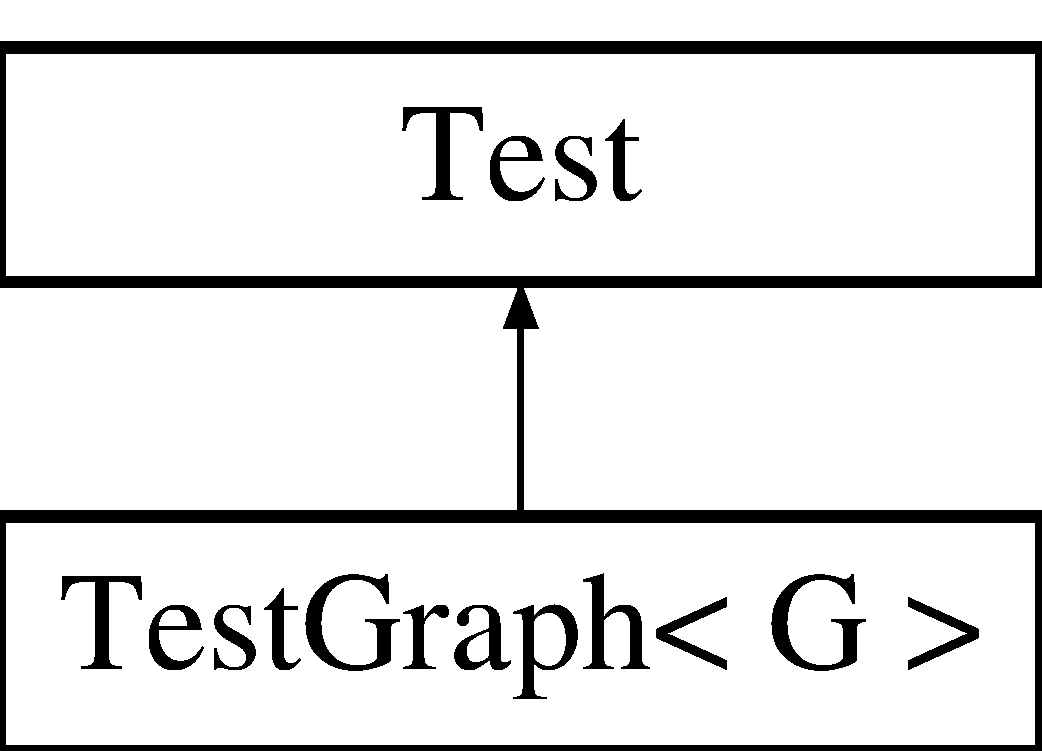
\includegraphics[height=2.000000cm]{structTestGraph}
\end{center}
\end{figure}
\subsection*{Public Types}
\begin{DoxyCompactItemize}
\item 
\hypertarget{structTestGraph_a149d9d185e2299b108590e2f83804351}{typedef G {\bfseries graph\-\_\-type}}\label{structTestGraph_a149d9d185e2299b108590e2f83804351}

\item 
\hypertarget{structTestGraph_ab66a56354d7a5751bf100ed3318bc498}{using {\bfseries vertex\-\_\-descriptor} = typename G\-::vertex\-\_\-descriptor}\label{structTestGraph_ab66a56354d7a5751bf100ed3318bc498}

\item 
\hypertarget{structTestGraph_a9cbf180f1275812b6162f30131bf55c3}{using {\bfseries edge\-\_\-descriptor} = typename G\-::edge\-\_\-descriptor}\label{structTestGraph_a9cbf180f1275812b6162f30131bf55c3}

\item 
\hypertarget{structTestGraph_a9ba4046e954f315bb4cf30cc93b07eac}{using {\bfseries vertex\-\_\-iterator} = typename G\-::vertex\-\_\-iterator}\label{structTestGraph_a9ba4046e954f315bb4cf30cc93b07eac}

\item 
\hypertarget{structTestGraph_a381ec62e5e7dd0855873bd39cd23683e}{using {\bfseries edge\-\_\-iterator} = typename G\-::edge\-\_\-iterator}\label{structTestGraph_a381ec62e5e7dd0855873bd39cd23683e}

\item 
\hypertarget{structTestGraph_a60336f93dc849f8acf2e8ac5c58785c3}{using {\bfseries adjacency\-\_\-iterator} = typename G\-::adjacency\-\_\-iterator}\label{structTestGraph_a60336f93dc849f8acf2e8ac5c58785c3}

\item 
\hypertarget{structTestGraph_a4b79f255258682679cad928f6d9bd8f1}{using {\bfseries vertices\-\_\-size\-\_\-type} = typename G\-::vertices\-\_\-size\-\_\-type}\label{structTestGraph_a4b79f255258682679cad928f6d9bd8f1}

\item 
\hypertarget{structTestGraph_a25d25458180a480adb3e05d404282f46}{using {\bfseries edges\-\_\-size\-\_\-type} = typename G\-::edges\-\_\-size\-\_\-type}\label{structTestGraph_a25d25458180a480adb3e05d404282f46}

\end{DoxyCompactItemize}


The documentation for this struct was generated from the following file\-:\begin{DoxyCompactItemize}
\item 
Test\-Graph.\-c++\end{DoxyCompactItemize}

%--- End generated contents ---

% Index
\newpage
\phantomsection
\addcontentsline{toc}{chapter}{Index}
\printindex

\end{document}
